% A basic LaTeX document for an assignment

% If you want the title to appear on a separate
% page, change notitlepage to titlepage
\documentclass[11pt,a4paper,notitlepage]{article}
\usepackage[utf8]{inputenc}
\usepackage[T1]{fontenc}
% If your hand-in is in icelandic change english to icelandic
% Note: This has nothing to do with Icelandic characters, they
% can always be used. This just tells other packages what 
% language you are using and changes the hyphenation used by LaTeX
% If icelandic is selected, a shorthand, "` and "', is also included
% for Icelandic quotation marks. They can also obtained by using 
% ,, and ``
\usepackage[english]{babel}
\usepackage{amsmath, amsthm, amssymb, amsfonts}
\usepackage{graphicx}
\usepackage{enumerate}
% To use the whole A4-page
% See: ftp://ftp.tex.ac.uk/tex-archive/macros/latex/contrib/geometry/geometry.pdf
% and http://en.wikibooks.org/wiki/LaTeX/Document_Structure
\usepackage{geometry}
% For header and footer
% See: ftp://ctan.tug.org/tex-archive/macros/latex/contrib/fancyhdr/fancyhdr.pdf
% and http://en.wikibooks.org/wiki/LaTeX/Document_Structure
\usepackage{fancyhdr}
% For prettier tables
% See: http://ctan.mackichan.com/macros/latex/contrib/booktabs/booktabs.pdf
% and  http://en.wikibooks.org/wiki/LaTeX/Tables
\usepackage{booktabs}


%%%%%%%%%%%%%%%%%%%%%%%%%%% SETUP %%%%%%%%%%%%%%%%%%%%%%%%%%%

% Set the margins of the paper. By default LaTeX uses huge margins
\geometry{includeheadfoot, margin=2.5cm}
% you can also use
% \geometry{a4paper}
% End of margins setup

% Setup header and footer
% Headers
\pagestyle{fancy} % To get the header and footer
\lhead{\small \textsc{Lab Exercises}}
\rhead{\small \textsc{Introduction to Electronic Engineering}}
% Footers
%\lfoot{Left footer text}
%\cfoot{\thepage} % This is the default behaviour
%\rfoot{Right footer text}

% If you don't want a line below the header or above the footer, 
% change the appropriate header/footerrulewidth to 0pt
\setlength{\headheight}{15.2pt} % This is set to avoid a warning
\renewcommand{\headrulewidth}{0.4pt}
\renewcommand{\footrulewidth}{0.4pt}
% End of header and footer setup

% Setup Problem/Solution environments
\theoremstyle{plain}
\newtheorem{problem}{Problem}[section]

\theoremstyle{remark}
\newtheorem*{solution}{Solution}
% End of Problem/Solution environments setup

%%%%%%%%%%%%%%%%%%%%%%%% END OF SETUP %%%%%%%%%%%%%%%%%%%%%%%%

\title{{\large \bf \MakeUppercase{Introduction to Electronic Engineering}} \\
		\large \textsc{Lab exercises}}

\author{\textsc{\small Antal János Monori \& Emil Már Einarsson }}

\begin{document}
	\maketitle
	
		\large \bf{\textsc{\section{Lab 1}}
	\begin{problem}
		Choose a 15K\(\Omega\) resistor. Read the color code and tolerance.
		\newline
		1. Measure the resistance using a multimeter.
		\newline
		2. Adjust the power supply on 5V. Connect the resistors to the power supply. Measure the voltage and the current of the resistor.
		\newline
		3. Repeat step two for 11 different voltages ranging from -15V to 15V.
		\newline
		4. Plot the I-V characteristics of the resistors. Are all measurements on one line? What is the slope of the line? Compare it with your readings of the code and tolerance as well as the multimeter readings. 
	\end{problem}

	\begin{solution}
		1. We measured the resistor to be 14.93K\(\Omega\).
		\newline
		2.Voltage: 5.15V and Amperage: 0.35 mA 
		\newline
		3. 
		\begin{table}[h]
			\begin{tabular}{| l | l | l | l | l | l | l | l | l | l | l | l |}
				\hline
				\textbf{Try} & 1 & 2 & 3 & 4 & 5 & 6 & 7 & 8 & 9 & 10 & 11 \\ \hline
				Voltage (V)  & -14.98 & -12.82 & -9.19 & -7.19 & -3.66 & 2.25 & 4.30 & 6.92 & 9.57 & 12.46 & 15 \\ \hline
				Current (mA) & -1.01 & -0.86 & -0.62 & -0.42 & -0.25 & 0.15 & 0.29 & 0.47 & 0.64 & 0.84 & 1.01 \\ \hline
			\end{tabular}
		\end{table}
		\newline
		4. 
		\begin{figure}[h!]
			\centering
			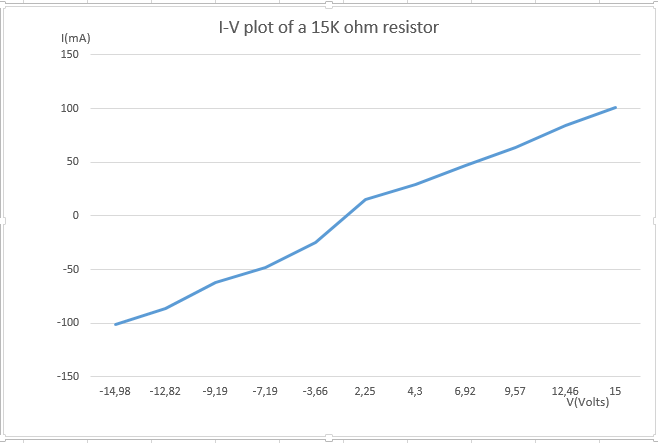
\includegraphics[width=0.5\textwidth]{images/ivplot.png}
		\end{figure}
	
		
	\end{solution}
	The slope is:
		$ (47 mA-29 mA)/(6.92 V-4.3 V)=6.87 mA/V $
	\clearpage
	\begin{problem}
		Choose the following resistors and construct each circuit given in the figure. \\
		R\(_{1}\): 15K\(\Omega\) \\
		R\(_{2}\): 22K\(\Omega\) \\
		R\(_{3}\): 33K\(\Omega\) \\
		R\(_{4}\): 10K\(\Omega\) \\
		\newline
		1. Calculate the equivalent resistance.
		\newline
		2. Measure the resistance of each indicated terminal using multimeter.
		\newline
		3. Are they different? Check out the tolerances and conclude why there is a difference.
		\begin{figure}[h!]
			\centering
			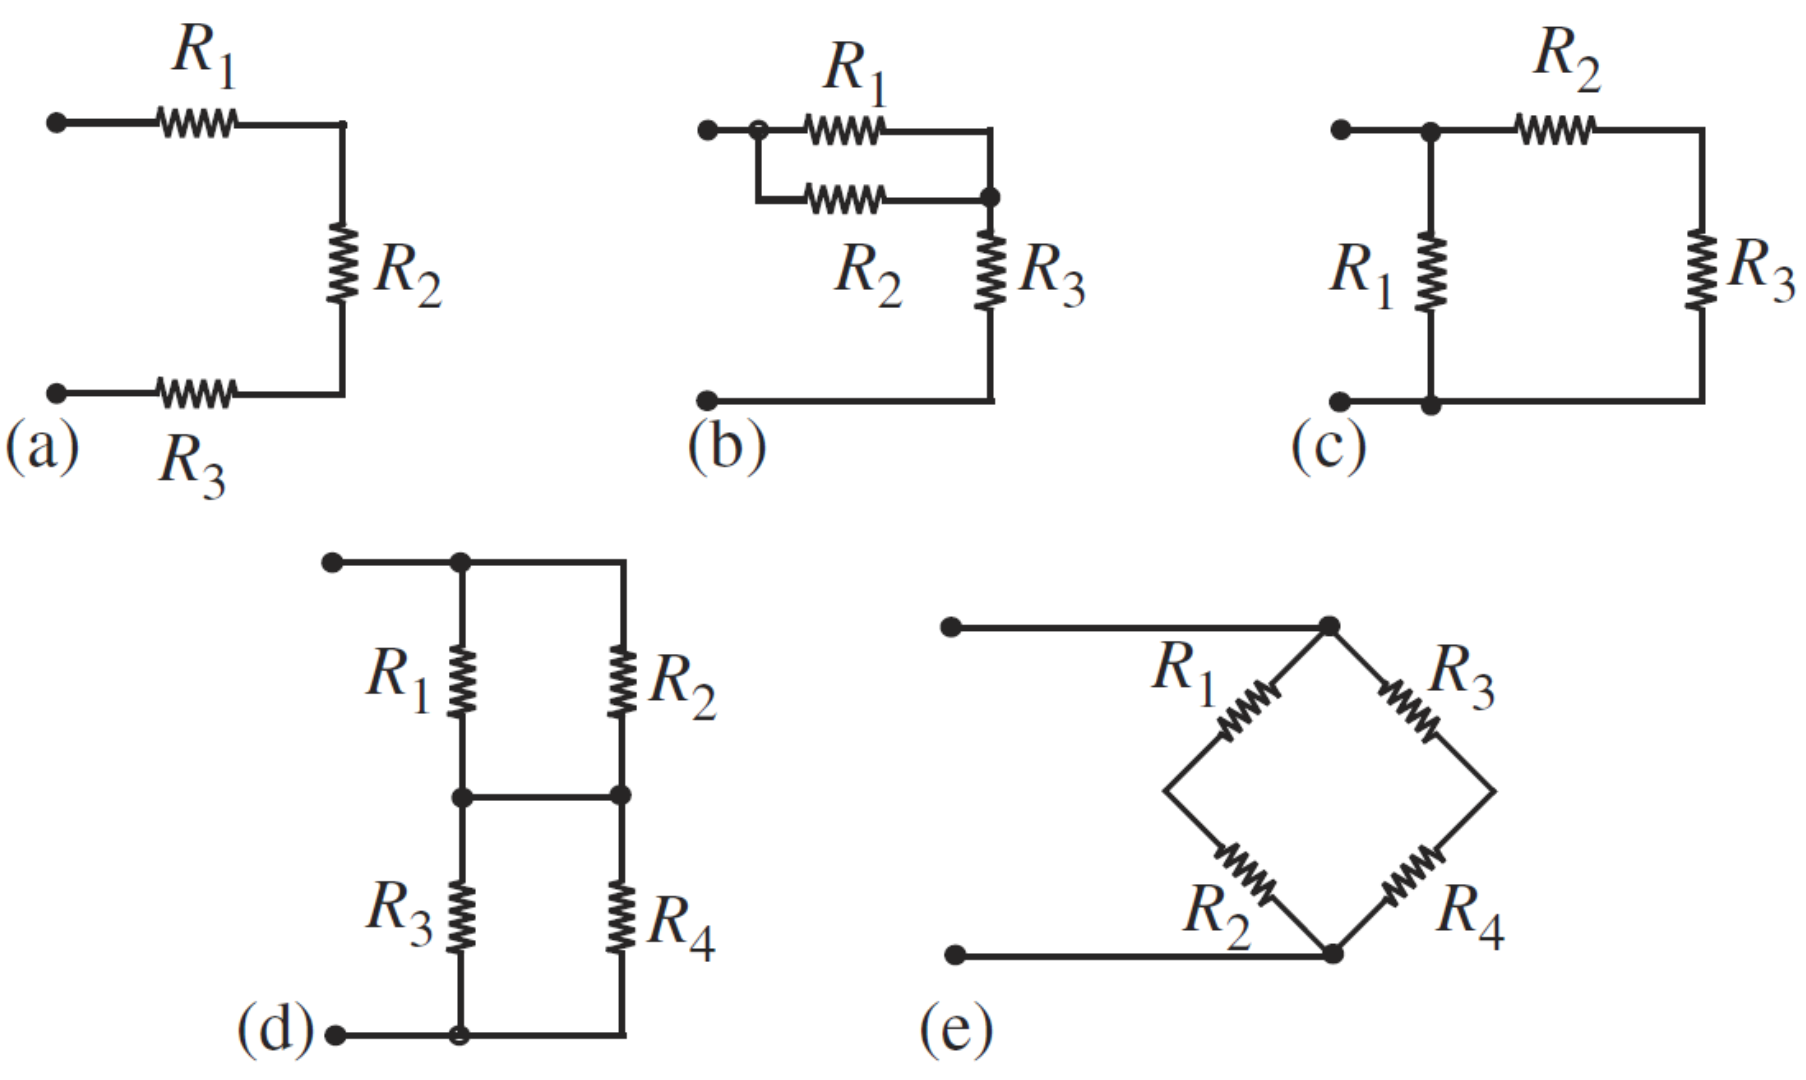
\includegraphics[width=0.5\textwidth]{images/figure1.png}
		\end{figure}
	\end{problem}
	
	\begin{solution}
		1. 
		(a) resistance is 70K\(\Omega\) \\
		(b) resistance is 41.91K\(\Omega\) \\
		(c) resistance is 11.78K\(\Omega\) \\
		(d) resistance is 16.59K\(\Omega\) \\
		(e) resistance is 19.88K\(\Omega\) \\
		\newline
		2. 
		(a) resistance is 69.8K\(\Omega\) \\
		(b) resistance is 41.7K\(\Omega\) \\
		(c) resistance is 11.73K\(\Omega\) \\
		(d) resistance is 16.55K\(\Omega\) \\
		(e) resistance is 19.8K\(\Omega\) \\
		\newline
		3. The average difference between measurements is (0.28+0.48+0.42+0.24+0.4)/5=0.36 percent. This is well within the 1 percent error the resistors are given for.
	\end{solution}
	\clearpage
	\begin{problem}
		Construct the circuit given in the following figure.
		\newline
		V\(_{A}\): 5V \\
		V\(_{B}\): 10V \\
		R\(_{1}\): 22K\(\Omega\) \\
		R\(_{2}\): 33K\(\Omega\) \\
		R\(_{3}\): 10K\(\Omega\) \\
		\newline
		1. Find all voltages and currents using KVL and KCL method.
		\newline
		2. Measure all currents and voltages stated in the circuit.
		\newline
		3. Compare the results.
		\begin{figure}[h!]
			\centering
			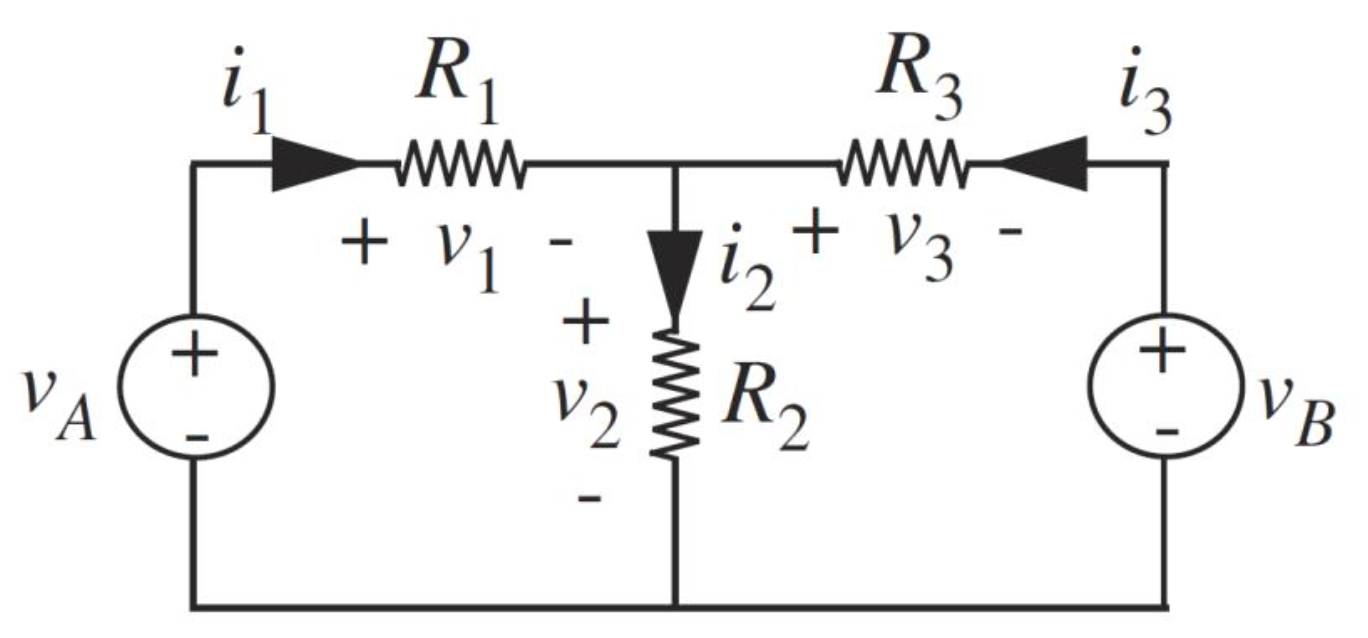
\includegraphics[width=0.2\textwidth]{images/circuit5.png}
		\end{figure}
	\end{problem}
	
	\begin{solution}
		\begin{figure}[h!]
				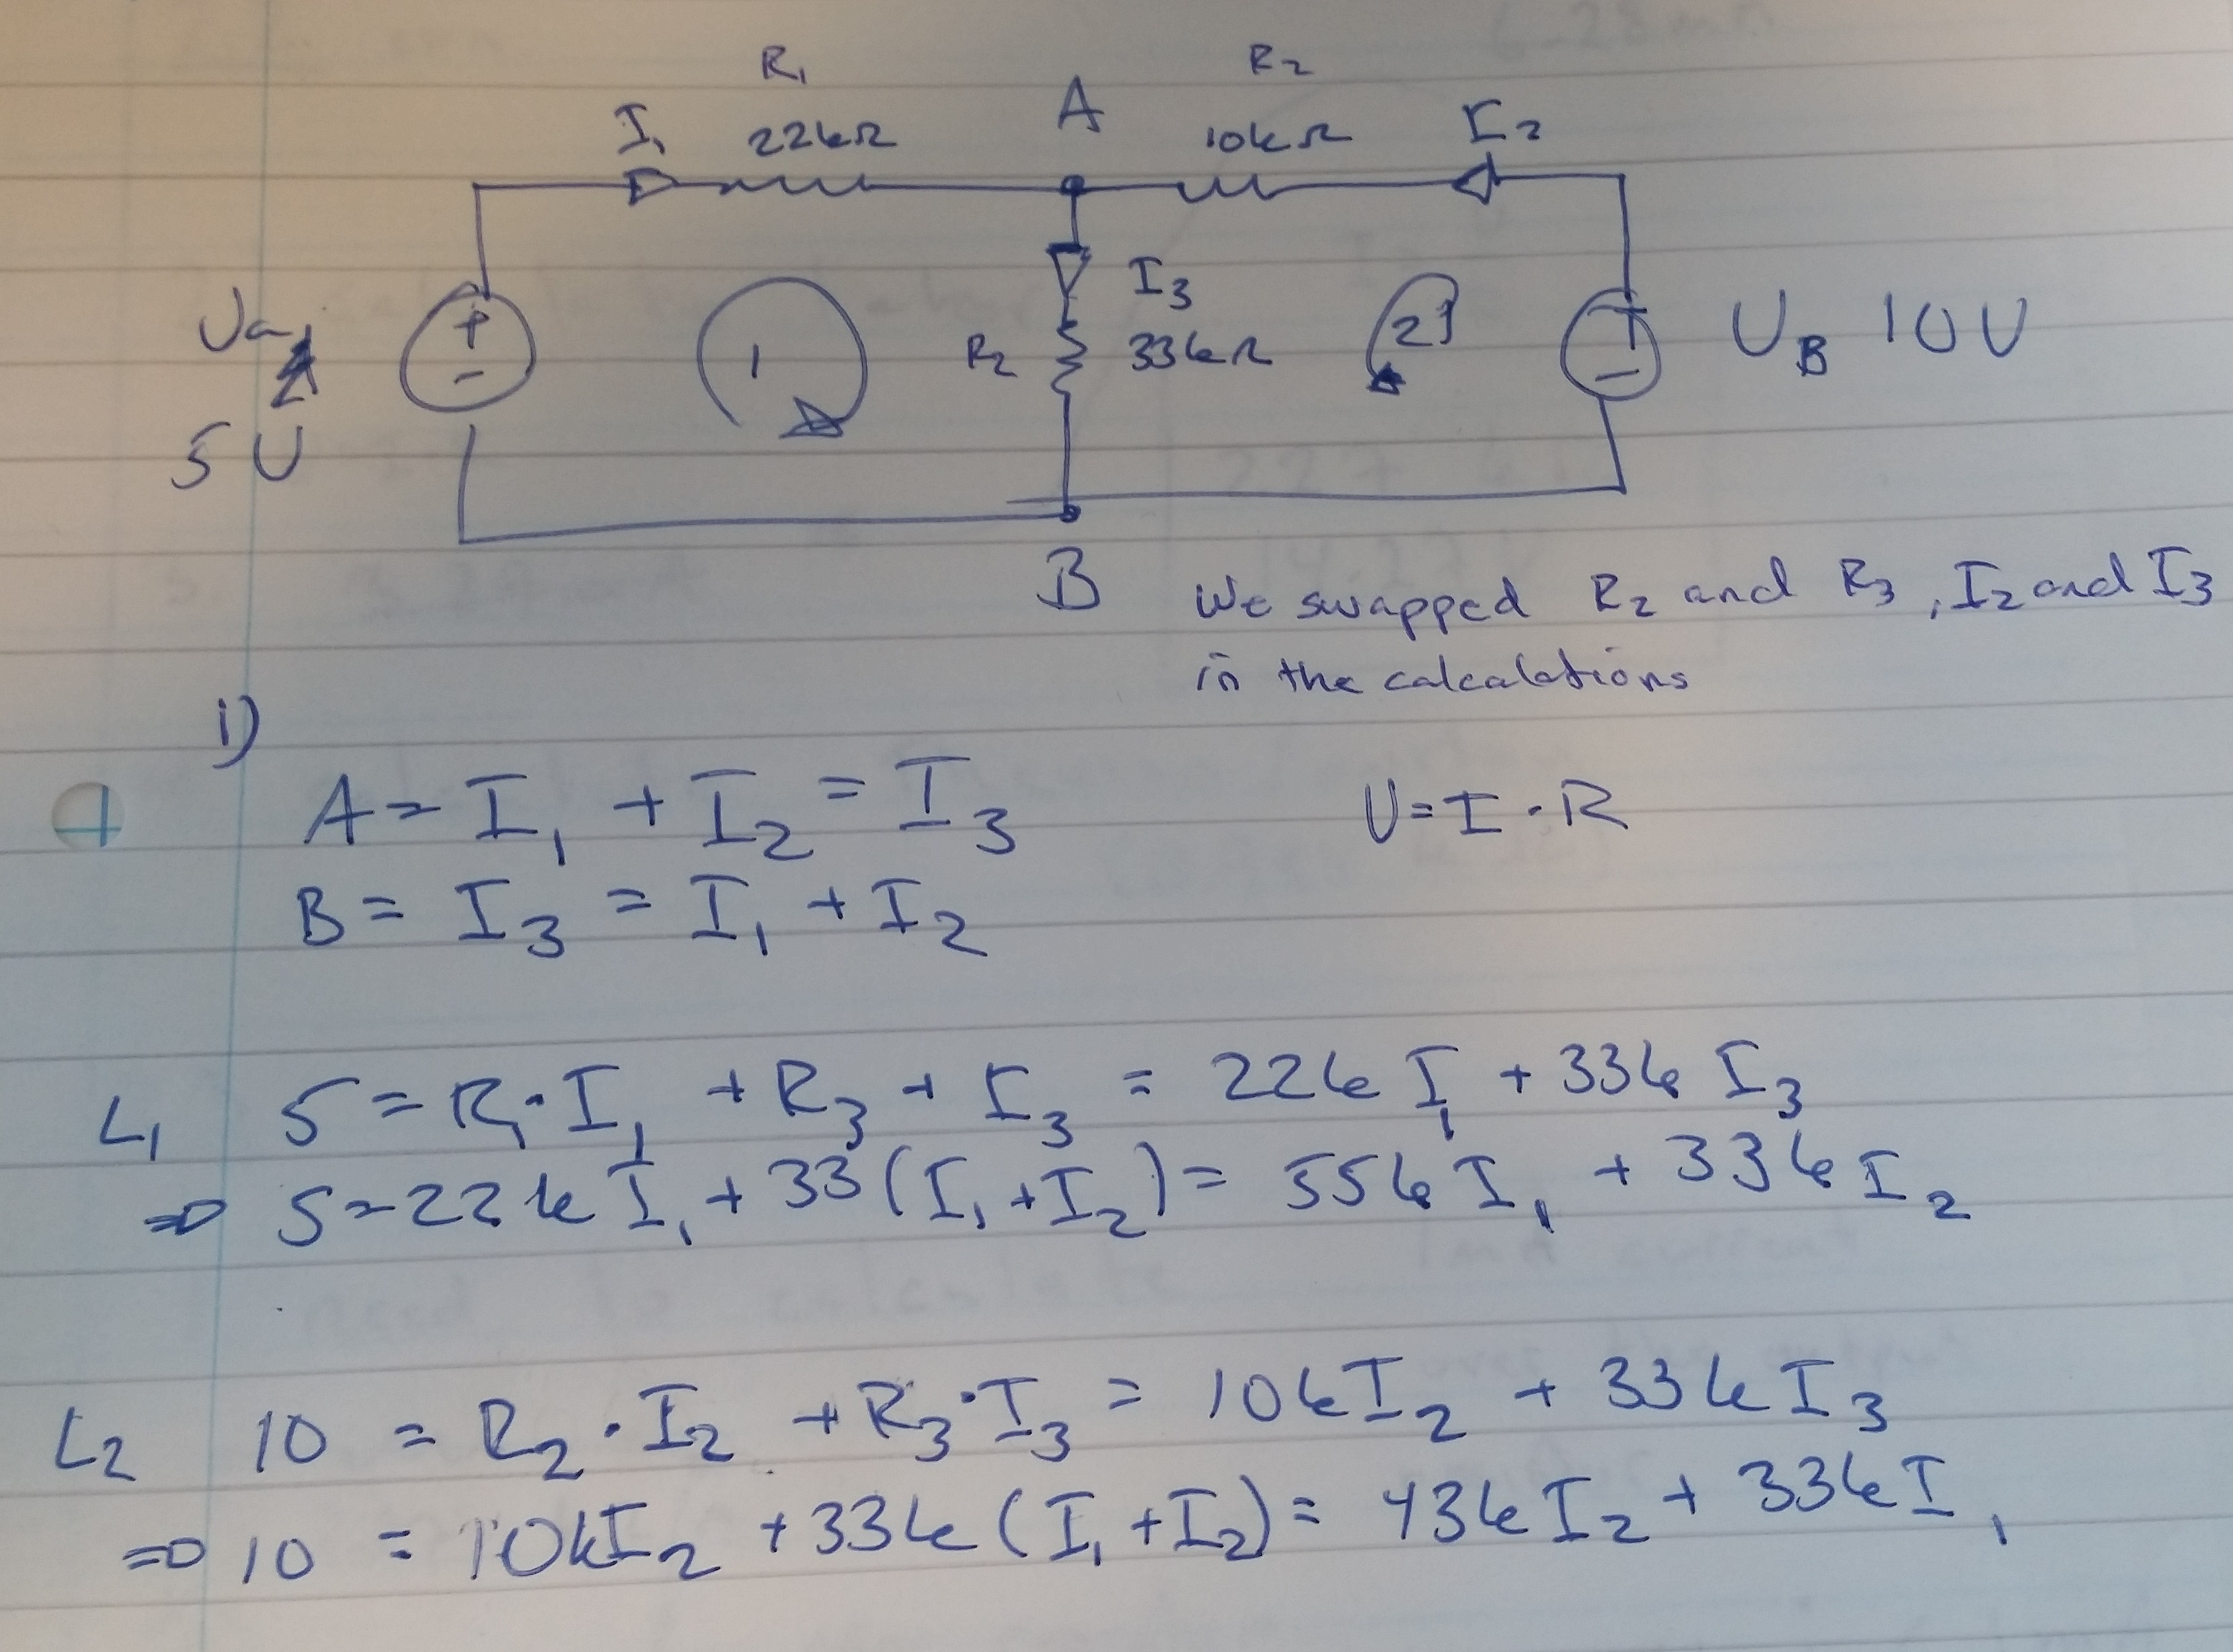
\includegraphics[width=0.6\textwidth]{images/lab1pic1.jpg}
		\end{figure}
		\begin{figure}[h!]
				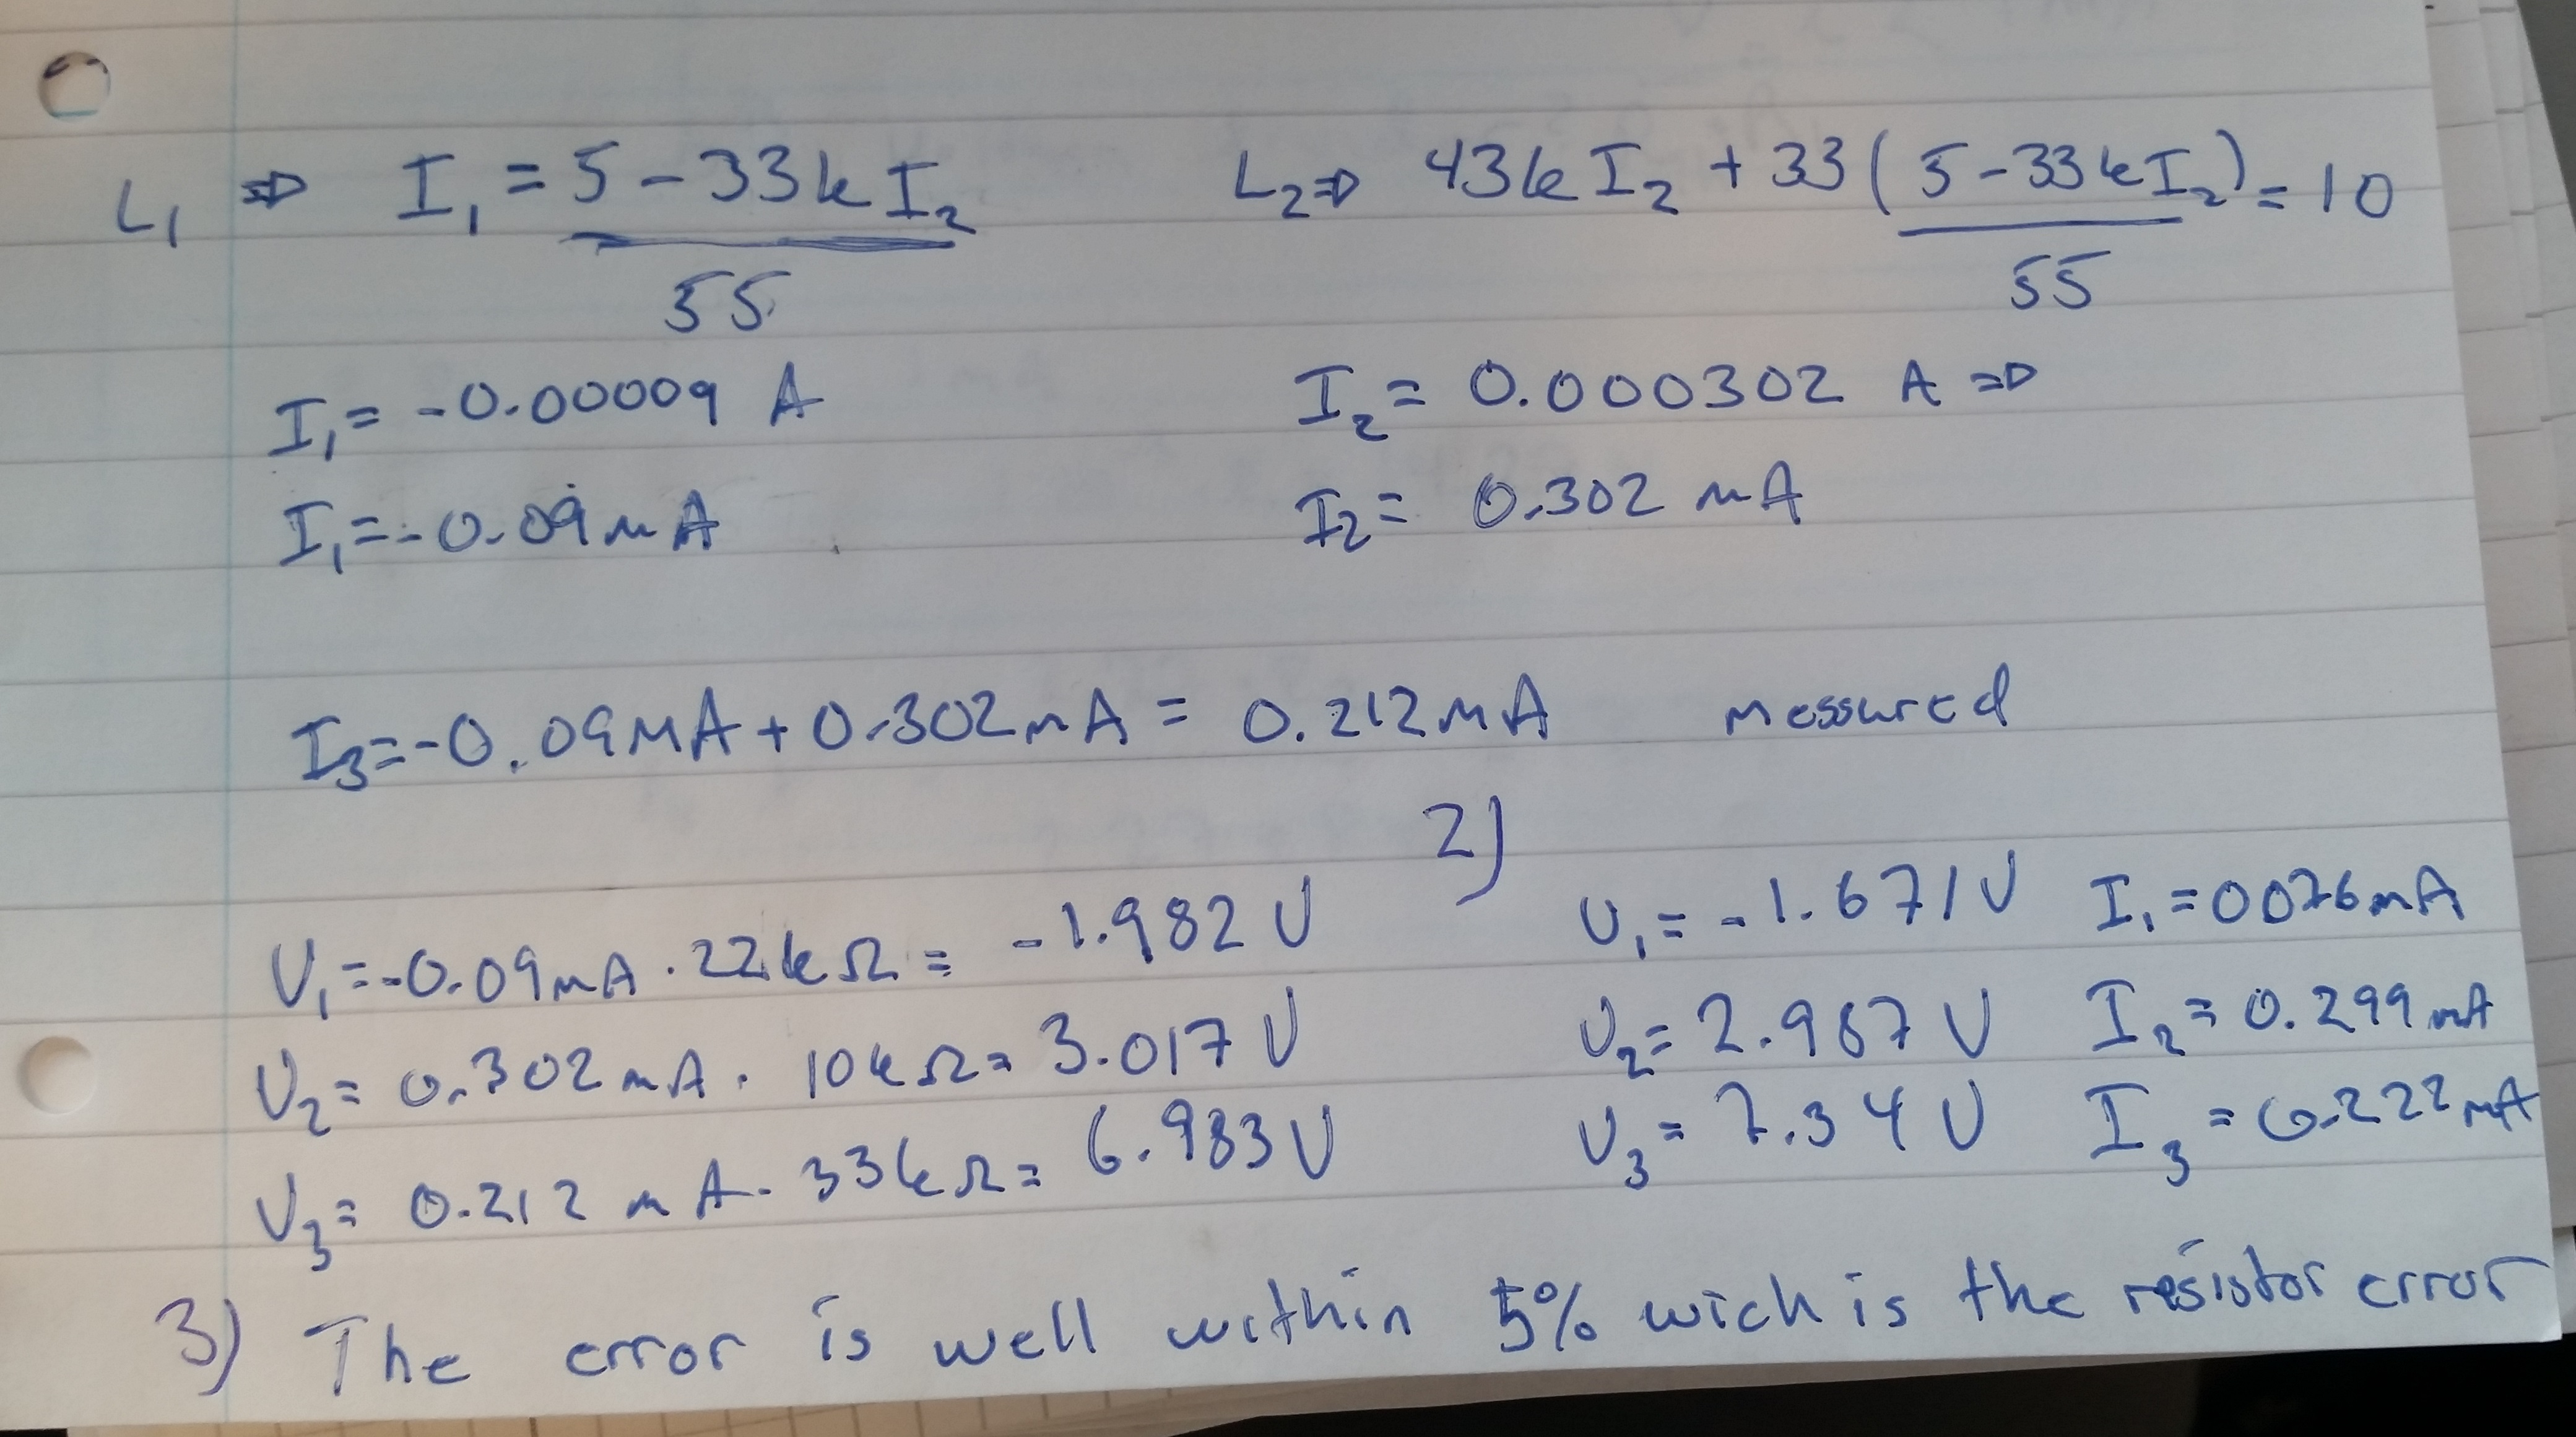
\includegraphics[width=0.6\textwidth]{images/lab1pic2.jpg}
		\end{figure}
	\end{solution}
	\clearpage	
	\begin{problem}
		Construct the circuit given in the following figure.
		\newline
		V\(_{A}\): 5V (with max current 60mA)\\
		I: 60mA (with max voltage 3V) \\
		R\(_{1}\): 180\(\Omega\) \\
		R\(_{2}\): 18\(\Omega\) \\
		R\(_{3}\): 270\(\Omega\) \\	
		\newline
		1. Calculate the voltage that falls on R\(_{3}\) using superposition.
		\newline
		2. Measure the voltage on R\(_{3}\).
		\newline
		3. Implement superposition in practice, by two tests (setting each source to zero and measuring the voltage)
		\newline
		4. Compare the results with your calculation.
		\newline
		5. Use the following resistors and explain why the measurements are not consistent with calculations\\
		R\(_{1}\): 180K\(\Omega\) \\
		R\(_{2}\): 18K\(\Omega\) \\
		R\(_{3}\): 270K\(\Omega\) \\	
		\begin{figure}[h!]
			\centering
			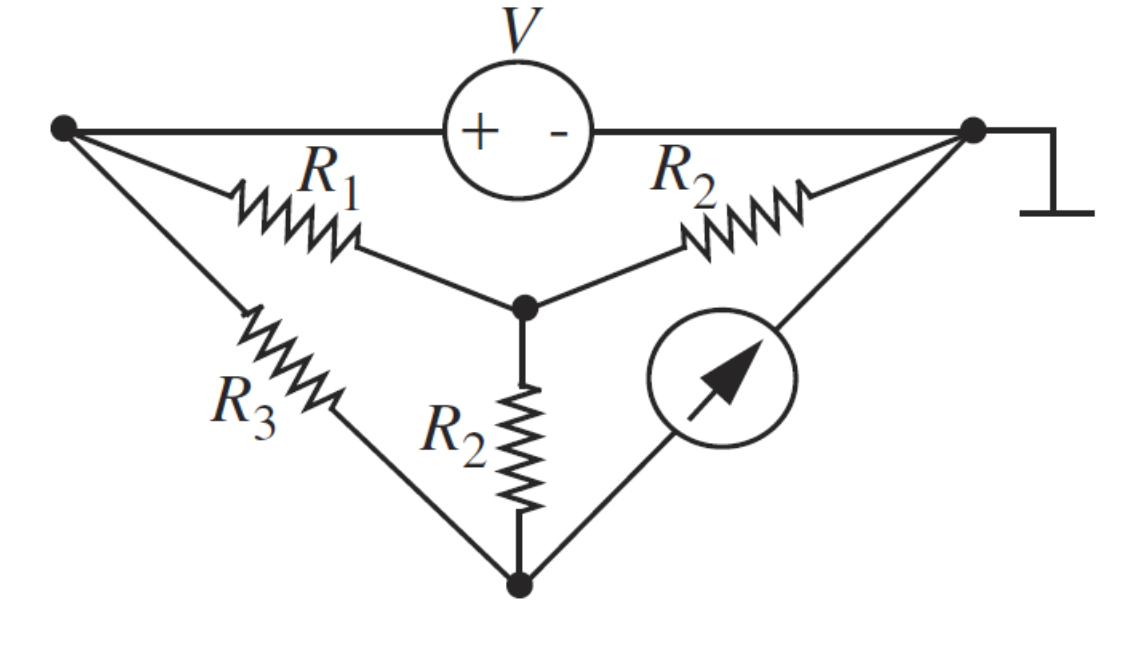
\includegraphics[width=0.3\textwidth]{images/circuit6.png}
		\end{figure}		
	\end{problem}
	
	\begin{solution}
		1.
		\begin{figure}[h!]
			\begin{subfigure}[H]{0.5\textwidth}
				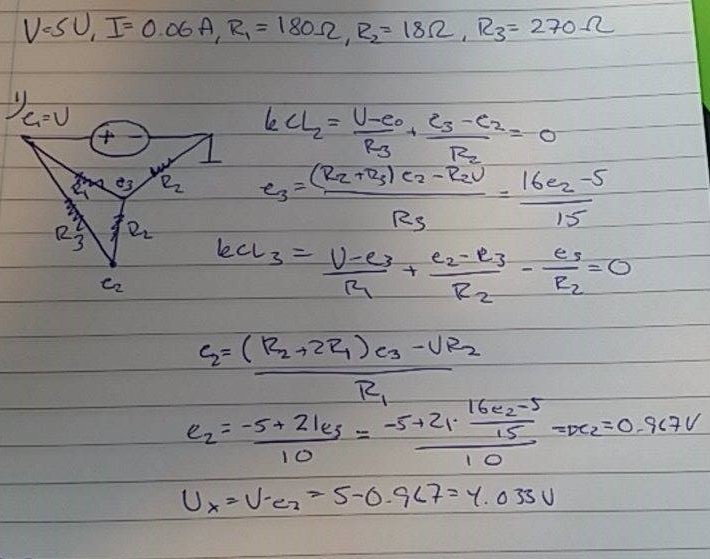
\includegraphics[width=0.8\textwidth]{images/lab3pic1.jpg}
				\subcaption{1.4.1}
			\end{subfigure}
			\begin{subfigure}[H]{0.7\textwidth}
				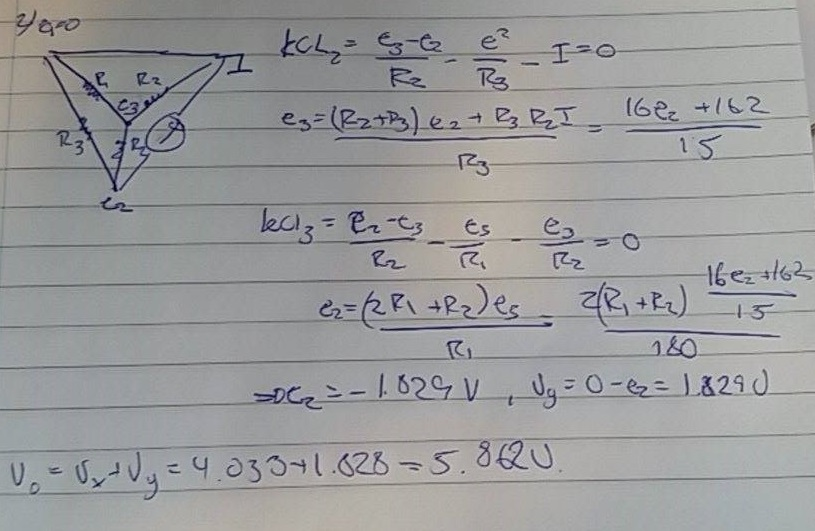
\includegraphics[width=0.7\textwidth]{images/lab3pic2.jpg}
				\subcaption{1.4.2}
			\end{subfigure}
		\end{figure}
		\newline
		2. R3= 5.59V
		\newline
		3. V1= 5.52, V2= 6mV, Total V= 5.58V
		\newline
		4. We calculated it to be 5.862V and measured it to be 5.8V.
		\newline
		5. I measured 8 V and said that the inconsistency is because in order to reach 60mA, we need a big voltage, so the current source reaches it's voltage limit and acts as a 3V voltage source.
	\end{solution}
	
	\pagebreak

		\large \bf{\textsc{\section{Lab 2}}
	\begin{problem}
		Problem 1 here.
	\end{problem}
	
	\begin{solution}
		Solution goes here.
	\end{solution}
	
	\begin{problem}
		Problem 1 here.
	\end{problem}
	
	\begin{solution}
		Solution goes here.
	\end{solution}
	
	\pagebreak
	
		\large \bf{\textsc{\section{Lab 3}}
	\begin{problem}
		Choose a diode type 1N4001 and build the following circuit.\\	
		R=100 \(\Omega\) (potentiometer) \\ 
		D is 1N4001 \\
		E=2v (max current I$_{max}$=350mA)
		\newline\newline
		1. Measure the diode and resistor voltage and current when changing the resistor R and fill the table
		\newline
		2. Plot the I-V characteristics  of the diode as well as the resistor. Are all measurements on one line? Are the components linear? Compare the diode i-v plot with the datasheet.
		
		\begin{figure}[h!]
			\centering
			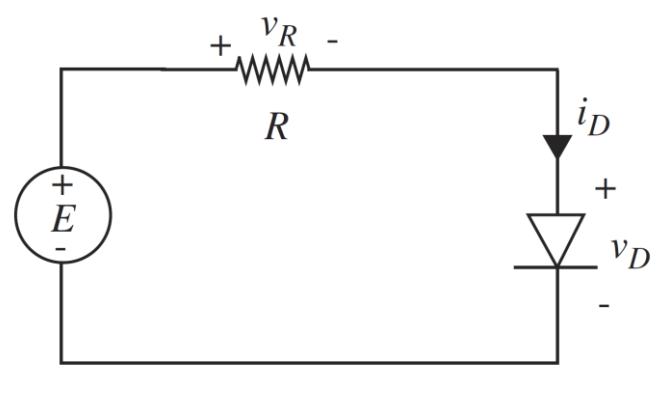
\includegraphics[width=0.5\textwidth]{images/circuit1.png}
		\end{figure}
	\end{problem}
	
	\begin{solution}
		1.
		\begin{table}[h]
			\begin{tabular}{| l | l | l | l | l | l | l | l | l | l | l | l |}
				\hline
				Try          & 1 & 2 & 3 & 4 & 5 & 6 & 7 & 8 & 9 & 10 & 11 \\ \hline
				R (\(\Omega\))   &   &   &   &   &   &   &   &   &   &    &    \\ \hline
				V$_{D}$ (V)  &   &   &   &   &   &   &   &   &   &    &    \\ \hline
				V$_{R}$ (V)  &   &   &   &   &   &   &   &   &   &    &    \\ \hline
				i$_{D}$ (mA) & 20 & 30 & 50 & 80 & 120 & 160 & 200 & 240 & 280 & 320 & 350 \\ \hline
			\end{tabular}
		\end{table}
		\newline
		2.
	\end{solution}
	\clearpage
	\begin{problem}
		In this exercise, we would like to build a full wave rectifier using a diode bridge.
		\newline
		1. Construct the following circuit using:\\
		R\(_{L}\)=10K\(\Omega\)\\
		D is 1N4001\\
		V\(_{i}\)=20sin(100\(\pi\)t)\\
		\newline
		2. Measure the input voltage and current using a multimeter.
		\newline
		3. Measure the output voltage on R\(_{L}\) using a multimeter and an oscilloscope.
		\newline
		4. Compare the measurements with your calculations
		\newline
		5. (Optional) Use a 470\(\mu\)F capacitor in parallel with R\(_{L}\) and measure the output voltage.
		\begin{figure}[h!]
			\centering
			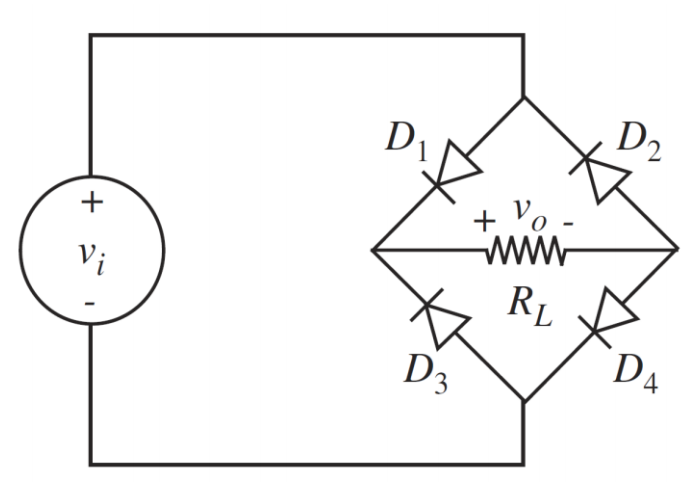
\includegraphics[width=0.5\textwidth]{images/circuit2.png}
		\end{figure}
	\end{problem}
	
	\begin{solution}
		1.
		\newline
		2.
		\newline
		3.
		\newline
		4.
		\newline
		5.
	\end{solution}
	\clearpage
	\begin{problem}
		Using an OpAmp TL082, construct an inverting amplifier of gain 2.
		\newline
		V\(_{i}\)=1.5v\\
		V\(_{CC}\)=12v\\
		Output current should not exceed 10mA
		\newline
		1. Measure the output voltage and compare with your expectations.
		\newline
		2. Use V\(_{i}\)=2sin(100\(\mu\)t) and measure the output voltage using an oscilloscope.
		\begin{figure}[h!]
			\centering
			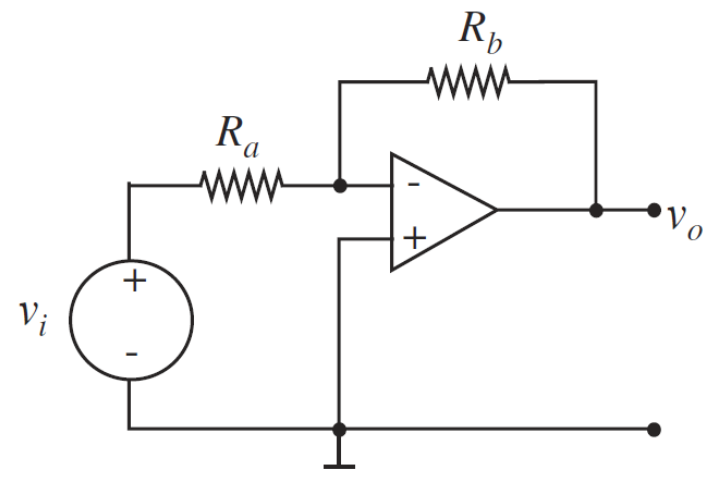
\includegraphics[width=0.5\textwidth]{images/circuit3.png}
		\end{figure}
	\end{problem}
	
	\begin{solution}
		1.
		\newline
		2.
	\end{solution}
	
	\pagebreak
	
	\large \bf{\textsc{\section{Lab 4}}
	\begin{problem}
		Using an OpAmp TL082, construct an amplifier that can deliver the following functions. Evaluate your circuit practically and theoretically.
		\newline
		1. z = 0.2x + y\\
		2. z = 3(x-y)\\
	\end{problem}
	
	\begin{solution}
		1. 
		\newline
		2. z = 3(x-y)
		
		x = 5V, y = 3V => 2*3=6V
	\end{solution}
	\clearpage
	\begin{problem}
		We would like to investigate the properties of the MOSFET type BS170. Construct the following circuit with R=1K\(\Omega\). (a and b are equivalent)
		\begin{figure}[h!]
			\centering
			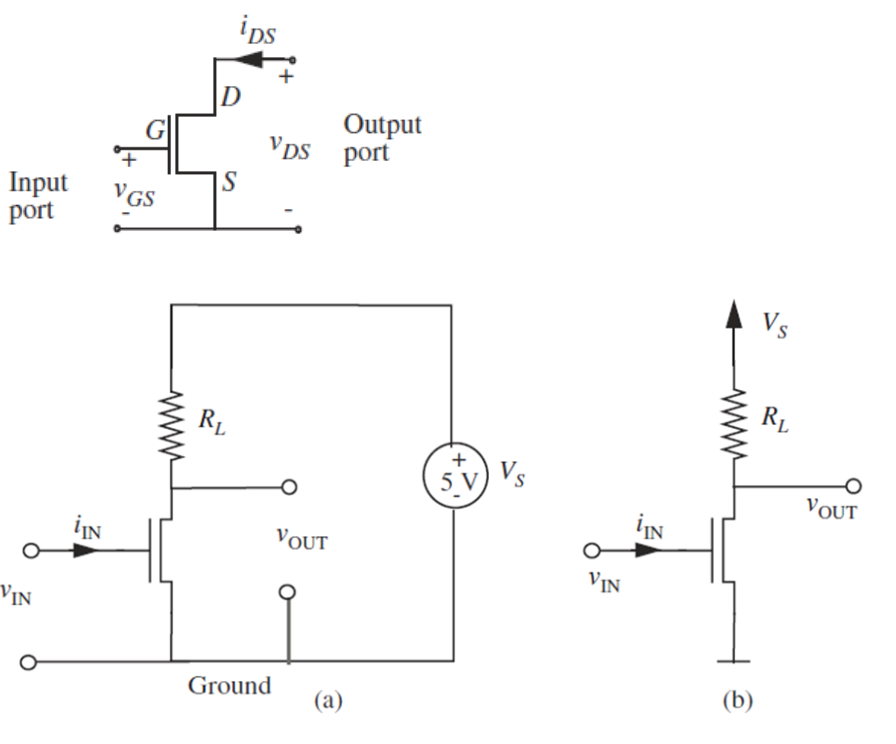
\includegraphics[width=0.5\textwidth]{images/circuit4.png}
		\end{figure}
		1. Measure the V\(_{out}\) and i\(_{DS}\) for the MOSFET for different values of V\(_{IN}\) and fill the table.
		\newline
		2. Plot your input-output characteristics of the MOSFET. What is the treshold voltage V\(_{T}\) for V\(_{GS}\)? Compare your findings with the datasheet.
		\newline
		3. Measure the V\(_{DS}\) and i\(_{DS}\) for the MOSFET for different values of V\(_{S}\) and fill the table \textbf{once the MOSFET is on}.
		\newline
		4. Plot the I-V characteristics of the MOSFET and obtain R\(_{ON}\). Compare your findings with the datasheet.
	\end{problem}
	
	\begin{solution}
		1. 		
		\begin{table}[h]
			\begin{tabular}{| l | l | l | l | l | l | l | l | l | l | l | l |}
				\hline
				Try & 1 & 2 & 3 & 4 & 5 & 6 & 7 & 8 & 9 & 10 & 11 \\ \hline
				V$_{OUT}$ (V) & 5 & 5 & 4.965 & 4.827 & 3.980 & 1.090 & 0.057 & 0.025 & 0.019 & 0.010 & 0.008 \\ \hline
				V$_{IN}$ (V) & 0 & 1 & 1.9 & 2.1 & 2.3 & 2.5 & 2.7 & 2.9 & 3 & 4 & 5 \\ \hline
			\end{tabular}
		\end{table}
		\newline
		2.
		\begin{figure}[h!]
			\centering
			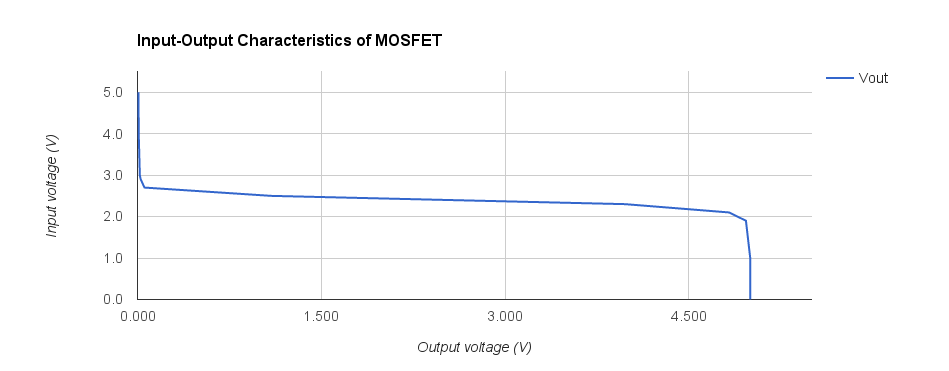
\includegraphics[width=0.6\textwidth]{images/plot422.png}
		\end{figure}
		\newline
		3.
		\begin{table}[h]
			\begin{tabular}{| l | l | l | l | l | l | l | l | l | l | l | l |}
				\hline
				Try & 1 & 2 & 3 & 4 & 5 & 6 & 7 & 8 & 9 & 10 & 11 \\ \hline
				V$_{OUT}$ (V) & 0.008 & 0.010 & 0.011 & 0.013 & 0.014 & 0.016 & 0.018 & 0.019 & 0.021 & 0.022 & 0.024 \\ \hline
				V$_{S}$ (V) & 5 & 6 & 7 & 8 & 9 & 10 & 11 & 12 & 13 & 14 & 15 \\ \hline
				i$_{DS}$ (mA) & 5 & 6 & 7 & 8 & 9 & 10 & 11 & 12 & 13 & 14 & 15 \\ \hline
			\end{tabular}
		\end{table}
		\newline
		4.
		\begin{figure}[h!]
			\centering
			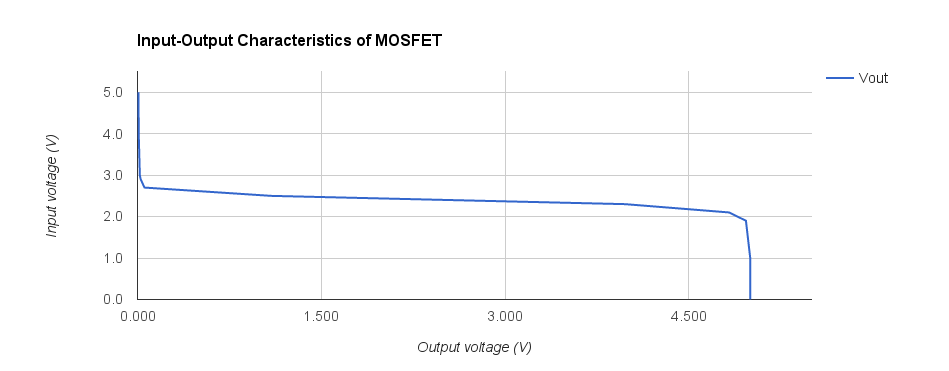
\includegraphics[width=0.6\textwidth]{images/plot422.png}
		\end{figure}
	\end{solution}
	\clearpage
	\begin{problem}
		Using MOSFET type BS170, construct circuits that represent the following logic functions. Evaluate your circuit practically and theoretically.
		\newline
		1. A+B+C \\
		2. A.B+\(\overline{C}\) \\
		3. A.B+C \\
		4. \(\overline{A.\overline{B}+\overline{C}}\)
	\end{problem}
	
	\begin{solution}
		1.
		\begin{figure}[h!]
			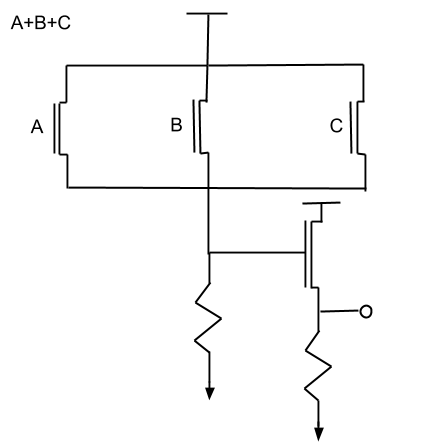
\includegraphics[width=0.18\textwidth]{images/solution431.png}
		\end{figure}
		\newline
		2.
		\begin{figure}[h!]
			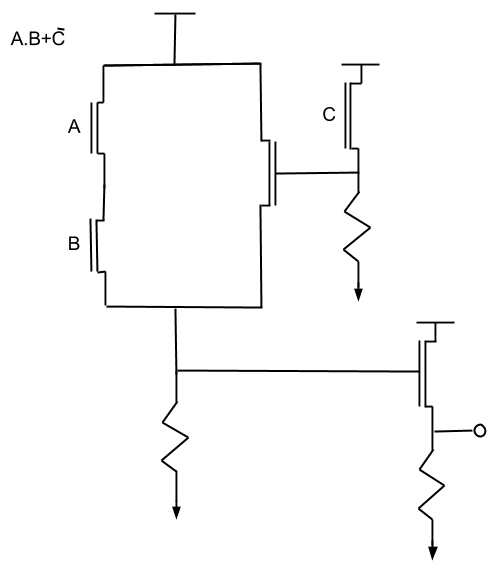
\includegraphics[width=0.18\textwidth]{images/solution432.png}
		\end{figure}
		\newline
		3.
		\begin{figure}[h!]
			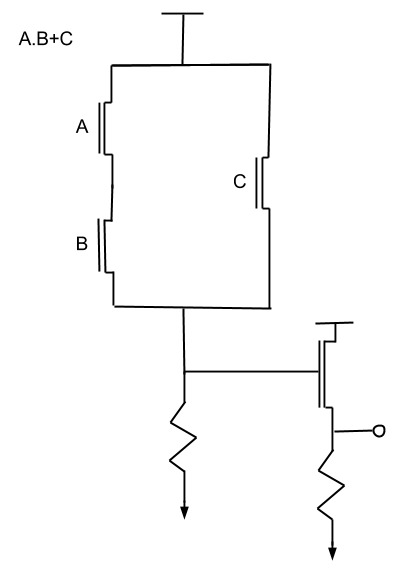
\includegraphics[width=0.18\textwidth]{images/solution433.png}
		\end{figure}
		\newline
		4.
		\begin{figure}[h!]
			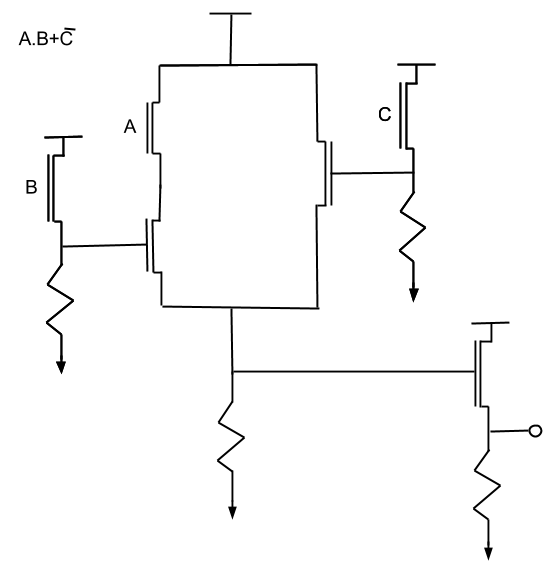
\includegraphics[width=0.18\textwidth]{images/solution434.png}
		\end{figure}
	\end{solution}
\end{document}

